We present the results of quantitative evaluations of XAI metrics to compare the Saliency Map method with other explanation methods on \otnn, and more generally compare XAI explanations methods on these networks and their unconstrained counterparts. On CelebA, we only present  the results for the label \textit{Mustache}, but results for the other labels are similar. Parameters for explanation methods and metrics are given in Appendix~A.4. We have chosen to present in Table \ref{table:xaimetric}  two SoTA XAI metrics that enable comparison between \otnn s~and unconstrained networks.  \textbf{$\mu\text{Fidelity}$ metric}~\cite{Bhatt20muFidelity} is a well-known method that measures the correlation between important variables defined by the explanation method and the model score decreases when these variables are reset to a baseline state (or replaced by uniform noise). Another important property for explanations is their stability for nearby samples. In~\cite{Yeh19InfidelityExplain}, the authors proposed Stability metrics based on the $L_2$ distance. To better evaluate this stability and make it comparable for different models, we replace the $L_2$ distance by $1-\rho$, $\rho$ being the Spearman rank correlation. Other model-dependent metrics are described in the Appendix. Results from the 50M parameter ResNet \otnn~are included in the human alignment study (Fig~\ref{fig:human_alignement}) to illustrate that enhancing the model's complexity can bolster both the accuracy and alignment. The following observations can be drawn from Table \ref{table:xaimetric}:
\iffalse
\subsubsection{Saliency Maps on \otnn~become reliable explanations}
\commentgreen{on s'etait fait critiqué sur des termes comme trusworrthy et reliable je pense qu'il faudrait changer ce titre de section: tentatives: \\
Enhanced scores for OTNNs Saliency Maps\\
%Good properties of OTNNs saleicy maps
\\
....
Ok vu tu supprime tout ca vu qu'il n'y a plus la tablleau
}
\fi

%\textbf{Insertion and Deletion metrics:} We first assess the quality of  Saliency Map explanations for the proposed network using Insertion and Deletion metrics~\cite{petsiuk18Rise}. Classical explanation methods, including the Saliency Map, are evaluated on CelebA and FashionMNIST datasets for both types of networks. Even if the score values cannot be compared between different networks, Table~\ref{tab:ins_del_metric} shows the Saliency Map method becomes competitive on these metrics and matches the top-ranking methods, whereas it is not the case for unconstrained networks. In Annex~\ref{ann:explanation_metrics}, we show that it is also the case for other metrics such as Robustness-SR~\cite{HsiehYLRKKH21}.

%\commentgreen{la parie deletion-insertion 0 c'est vraiment pas clair je pense qu'il faut l'enlever. On peut remplacer par robustnessSR si on arrive a faire FashionMNIST}.

% \iffalse
% \fel{Proposition: j'ai corrigé quelques typos dans la table et essayé de séparer des parties. Je ne suis pas sur que ce soit mieux, je laisse les deux et vous choisirez ;)}
% \begin{table}
%   \caption{Insertion and Deletion metrics evaluation; GC: GradCam, GI: Gradient.Input, IG: Integrated Gradient, Saliency Rk : Rank}
%   \label{tab:ins_del_metric_2}
%   \centering
%   \begin{tabular}{lc|cccccc}
%     \toprule
% Dataset& Network&  \multicolumn{6}{c}{Deletion-Uniform (lower is better)}  \\
% & & GC & GI & IG & Rise& Saliency& SmoothGrad\\
%  \midrule
% CelebA& \otnn & 9.41& 9.38& 9.36& 8.89& 8.32 (Rk2) & \textbf{8.28}\\
% & Unconstrained& 5.13& 3.33& \textbf{3.18}& 3.61& 3.50 (Rk4) & 3.41\\
% Fashion-& \otnn& 0.23& 0.28& 0.28& 0.24& 0.22 (Rk2) & \textbf{0.21}\\
% MNIST & Unconstrained& 0.32& 0.35& 0.39& 0.32& 0.26 (Rk2) & \textbf{0.24}\\
%  \midrule
% & &  \multicolumn{6}{c}{Insertion Uniform (higher is better)} \\
% CelebA& \otnn& 10.25& 10.44& 10.50& 10.46& \textbf{11.29} (Rk1) & 11.28\\
% & Unconstrained& 9.43& 8.45& 9.24& \textbf{12.20} & 6.71 (Rk6) & 6.72\\
% Fashion-& \otnn& \textbf{0.28}& 0.20& 0.20& 0.26& 0.25 (Rk4) & 0.26\\
% MNIST & Unconstrained& \textbf{0.44} & 0.32& 0.26& 0.40& 0.30 (Rk4)& 0.24\\
%     \bottomrule
%     \end{tabular}
% \end{table}
% \fi 



\textbf{Saliency Map on \otnn s exhibit more fidelity and stability : } 
We confirm and amplify the results in ~\cite{felHowGood22}. Table.~\ref{table:xaimetric} clearly states that 
%Table.~\ref{table:xaimetric} confirms and amplifies the results in ~\cite{felHowGood22}, clearly stating that 
for most of the explanation methods, the $\mu\text{Fidelity}$,  zero or uniform, is significantly higher for \otnn s. And above all, Saliency Map score for \otnn s~is always higher than any other attribution method score for unconstrained models.
%whatever the explanation method, the $\mu\text{Fidelity}$, with zero or uniform score modification, is significantly higher when it is applied on \otnn. There are instances where this is not the case for the ResNet architecture; however, in such cases, the Saliency Map of OTNN significantly outperforms any attribution metrics for unconstrained models. 
%This confirms and amplify the result ~\cite{felHowGood22}, which shows that \onlyonelip~ neural networks, for the two proposed metrics, produce explanations with higher scores than common neural networks (\mathieu{A améliorer}). 
A similar observation 
holds for 
%applies to 
the Stability Spearman rank
: \otnn~scores are better whatever the attribution method.
%, where the score is substantially better for \otnn, regardless the attribution considered.


\textbf{Saliency Map method on \otnn s~is equivalent to other attribution methods: }
We observe that the scores from the Saliency Maps and other methods are very similar for \otnn, with Saliency Maps consistently ranking among the top attribution methods. For the unconstrained case, Saliency Maps are occasionally outperformed by other attribution methods. Notably, for the ResNet architecture, attribution methods other than Saliency Maps and GradCAM yield more erratic results for fidelity metrics. To highlight these results, we compare the $L_2$ distance between Saliency Maps and SmoothGrad explanations, as suggested by \cite{Adebayo18Sanity,felHowGood22,tomsett2019sanity,ghorbani2017interpretation}. The explanation distances for \otnn~are significantly lower than for the unconstrained ones and closely approach zero, indicating that for \otnn, averaging over a large set of noisy inputs—as in SmoothGrad—is unnecessary. This is illustrated in Fig.\ref{fig:saliency_smoothgrad}.
\iftrue
\begin{figure*}
\begin{tabular}{@{}c@{}cc@{}}
\centering
    \begin{tabular}{c}
  \rowcolor{white}  \rotatebox{90}{\textbf{Saliency}}
  \end{tabular} & 
  \begin{tabular}{@{}l@{}l@{}l@{}}
    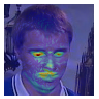
\includegraphics[width=.16\linewidth]{img/saliency_smoothgrad/saliency_1Lip_3_crop.png} &
  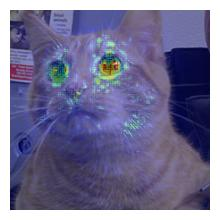
\includegraphics[width=.16\linewidth]{img/catvsdog/OTNN_saliency_1.jpg} & 
  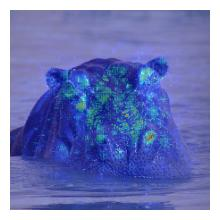
\includegraphics[width=.16\linewidth]{img/imagenet/OTNN_saliency_2.jpg}
  \end{tabular} & 
  \begin{tabular}{@{}l@{}l@{}l@{}}
  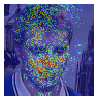
\includegraphics[width=.16\linewidth]{img/saliency_smoothgrad/saliency_Unconst_3_crop.png} &
  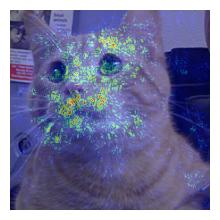
\includegraphics[width=.16\linewidth]{img/catvsdog/resnet50_saliency_1.jpg} & 
  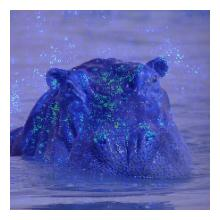
\includegraphics[width=.16\linewidth]{img/imagenet/resnet50_saliency_2.jpg}
  \end{tabular}\\

  \begin{tabular}{l}
   \rotatebox{90}{\textbf{SmoothGrad}} 
  \end{tabular} &
  \begin{tabular}{@{}l@{}l@{}l@{}} 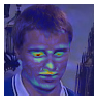
\includegraphics[width=.15\linewidth]{img/saliency_smoothgrad/smoothgrad_1Lip_3_crop.png} &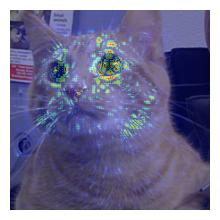
\includegraphics[width=.16\linewidth]{img/catvsdog/OTNN_smooth_1.jpg} & 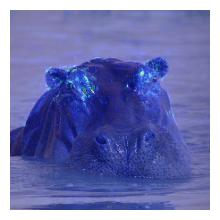
\includegraphics[width=.16\linewidth]{img/imagenet/OTNN_smooth_2.jpg}
  \end{tabular} & 
  \begin{tabular}{@{}l@{}l@{}l@{}}
  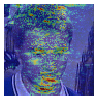
\includegraphics[width=.16\linewidth]{img/saliency_smoothgrad/smoothgrad_Unconst_3_crop.png} & 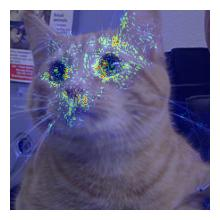
\includegraphics[width=.16\linewidth]{img/catvsdog/resnet50_smooth_1.jpg} & 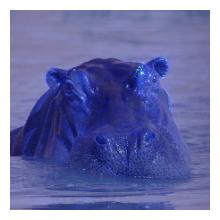
\includegraphics[width=.16\linewidth]{img/imagenet/resnet50_smooth_2.jpg}
  \end{tabular}\\
& (a)~\otnn
  &  (b) Unconstrained
\end{tabular}
\caption{Comparison of Saliency Map and SmoothGrad  explanations for (a) \otnn~ and (b) unconstrained network for, from left to right, CelebA, Cat vs Dog and Imagenet datasets.} %\commentgreen{Thomas a donné des nouvelles images elles sont dans saliency_smoothgrad/robust... a mettre en annexe ou ici }}
\label{fig:saliency_smoothgrad}
\end{figure*}
\fi

\iffalse
\begin{figure*}
\begin{tabular}{@{}c@{}c@{}c}
\centering
  \begin{tabular}{l}
    \rotatebox{90}{\textbf{Saliency}}
  \end{tabular}
 & 
  \begin{tabular}{@{}l@{}l@{}l}
    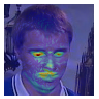
\includegraphics[width=.14\linewidth]{img/saliency_smoothgrad/saliency_1Lip_3_crop.png} &
  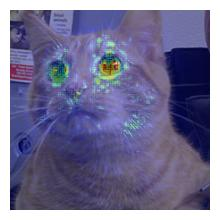
\includegraphics[width=.15\linewidth]{img/catvsdog/OTNN_saliency_1.jpg} %& 
%  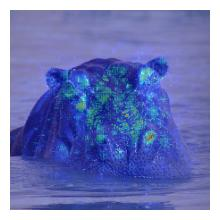
\includegraphics[width=.15\linewidth]{img/imagenet/OTNN_saliency_2.jpg}
  \end{tabular} &
  \multirow{6}{c}{\includegraphics[width=.35\textwidth]{img/human_alignment.jpg}}
  \\

  \begin{tabular}{l}
   \rotatebox{90}{\textbf{SmoothGrad}} 
  \end{tabular} &
  \begin{tabular}{@{}l@{}l@{}l} 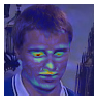
\includegraphics[width=.14\linewidth]{img/saliency_smoothgrad/smoothgrad_1Lip_3_crop.png} &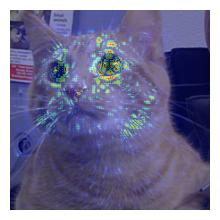
\includegraphics[width=.15\linewidth]{img/catvsdog/OTNN_smooth_1.jpg} %& 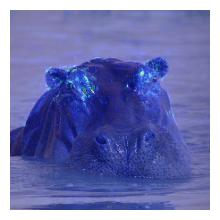
\includegraphics[width=.15\linewidth]{img/imagenet/OTNN_smooth_2.jpg}
  \end{tabular} &  \\
& (a)~\otnn  & \\
  \begin{tabular}{l}
    \rotatebox{90}{\textbf{Saliency}}
  \end{tabular}
 & 
  \begin{tabular}{@{}l@{}l@{}l}
  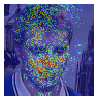
\includegraphics[width=.15\linewidth]{img/saliency_smoothgrad/saliency_Unconst_3_crop.png} &
  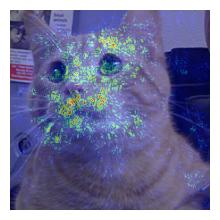
\includegraphics[width=.16\linewidth]{img/catvsdog/resnet50_saliency_1.jpg} %& 
%  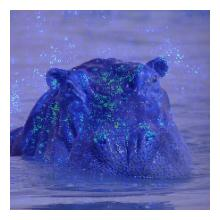
\includegraphics[width=.15\linewidth]{img/imagenet/resnet50_saliency_2.jpg}
  \end{tabular}  & \\
  \begin{tabular}{l}
   \rotatebox{90}{\textbf{SmoothGrad}} 
  \end{tabular} &
  \begin{tabular}{@{}l@{}l@{}l}
  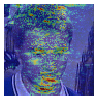
\includegraphics[width=.15\linewidth]{img/saliency_smoothgrad/smoothgrad_Unconst_3_crop.png} & 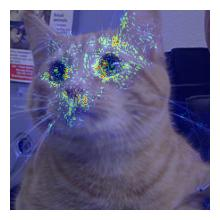
\includegraphics[width=.16\linewidth]{img/catvsdog/resnet50_smooth_1.jpg} %& 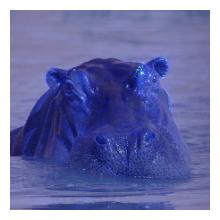
\includegraphics[width=.15\linewidth]{img/imagenet/resnet50_smooth_2.jpg}
  \end{tabular} & \\
&   (b) Unconstrained& 
\end{tabular}
\caption{Comparison of Saliency Map and SmoothGrad  explanations for (a) \otnn~ and (b) unconstrained network for the respectively CelebA, cat vs dog and imagenet.} %\commentgreen{Thomas a donné des nouvelles images elles sont dans saliency_smoothgrad/robust... a mettre en annexe ou ici }}
\label{fig:saliency_smoothgrad}
\end{figure*}
\fi
%\textbf{Saliency Map on \otnn~are less complex:} 
%Complexity of a given explanation is linked to the understandability by a human. \commentgreen{Thomas si tu as des references ? TBC should be kolmogorov but JPEG is a good surrogate}
%Inspired by previous works~\cite{da2011image} highlighting a strong correlation between Kolmogorov complexity and human evaluation of complexity~\cite{forsythe2008confounds,forsythe2009visual}. We used a JPEG based compressor~\cite{vereshchagin2005lossy} as a simple approximation of  visual explanation complexity~\cite{li2004similarity}: \otnn s~yield simpler explanations than unconstrained networks in all case. %($16.8kB$) -see Figure~\ref{fig:saliency_smoothgrad} for a qualitative comparison-.
%. \commentgreen{il manque les resultats (a faire Franck)}



%\subsubsection{\otnn s~ provide better explanations}
%\commentgreen{idem better ca veut pas dire grand chose\\
%\otnn s~ explanations exhibit more fidelity and stability\\
%...\\
%d'autres propositions?}





\textbf{\otnn s~ explanations are aligned with human ones : }
Adopting the method presented in~\cite{linsley2017visual}, using the ClickMe dataset, we follow strictly their experimental methodology and use their code\footnote{https://github.com/serre-lab/Harmonization} to compute the human feature alignment of OTNN Saliency Maps and compare with the others models tested in ~\cite{ fel2022aligning}-- more than 100 recent deep neural networks. In Figure ~\ref{fig:human_alignement}, we demonstrate that 
OTNN models Saliency Maps, %the Saliency Map of  the OTNN model,
which also carries a theoretical interpretation as the direction of the transport plan,  is more aligned with human attention than any other tested models and significantly surpasses the Pareto front discovered by~\cite{fel2022aligning}. The OTNN model is even more aligned than a ResNet50 model trained with a specific alignment objective, proposed by~\cite{fel2022aligning}, and called \textit{Harmonized ResNet50}. 
This finding is interesting as it indicates \otnn s are less prone to relying on spurious correlations~\cite{geirhos2020shortcut} and 
%is more adept at capturing 
better capture
human visual strategies for object recognition.
%The implications of these findings are crucial first for cognitive science: A model with closer alignment with human attention and visual strategies can provide a more comprehensive understanding of how vision operates for humans. Besides, it enhances the predictability, interpretability, and performance of object recognition models which as positive consequences in industry settings.
The implications of these results are crucial for both cognitive science and industrial applications. A model that more closely aligns with human attention and visual strategies can provide a more comprehensive understanding of how vision operates for humans, and also enhance the predictability, interpretability, and performance of object recognition models in industry settings. 
Furthermore, the drop in alignment observed in recent models highlights the necessity of considering the alignment of model visual strategies with human attention while developing object recognition models to reduce the reliance on spurious correlations and ensure that our models get things right for the right reasons.

\iftrue
\begin{figure*}
\centering
\includegraphics[width=1.\textwidth]{img/human_alignment_flat_2.pdf}
\caption{\textbf{\otnn~are aligned with Human attention.} Our study shows that the Saliency Map of OTNN model is highly aligned with human attention.% This finding is supported by the work of~\cite{fel2022aligning}, which demonstrates the trade-off between deep neural network (DNN) performance and alignment with human feature importance from the ClickMe~\cite{linsley2017visual} dataset. The degree of alignment between human and DNN saliency is measured using the mean Spearman correlation, normalized by the average inter-rater alignment of humans. 
%Among the hundreds of model tests performed in the original study, our model is the only one that breaks the Pareto front, suggesting a superior trade-off between DNN performance and alignment with human attention. Even an Harmonized model from~\cite{fel2022aligning} study, which was specifically designed to predict human attention, achieves a lower alignment than our model. \fel{on peut remove ca si vous voulez:} Overall, our results highlight the potential of the OTNN model to capture the visual strategies used by humans for object recognition, and may lead to improved performance and interpretability of object recognition models in both cognitive science and industry applications.
}
\label{fig:human_alignement}
\end{figure*}
\fi



\iffalse
\begin{figure*}
\centering
\includegraphics[width=.7\textwidth]{img/human_alignment.jpg}
\caption{\textbf{\otnn~are aligned with Human attention.} Our study shows that the Saliency Map of \otnn~model is highly aligned with human attention.% This finding is supported by the work of~\cite{fel2022aligning}, which demonstrates the trade-off between deep neural network (DNN) performance and alignment with human feature importance from the ClickMe~\cite{linsley2017visual} dataset. The degree of alignment between human and DNN saliency is measured using the mean Spearman correlation, normalized by the average inter-rater alignment of humans. 
%Among the hundreds of model tests performed in the original study, our model is the only one that breaks the Pareto front, suggesting a superior trade-off between DNN performance and alignment with human attention. Even an Harmonized model from~\cite{fel2022aligning} study, which was specifically designed to predict human attention, achieves a lower alignment than our model. \fel{on peut remove ca si vous voulez:} Overall, our results highlight the potential of the OTNN model to capture the visual strategies used by humans for object recognition, and may lead to improved performance and interpretability of object recognition models in both cognitive science and industry applications.
}
\label{fig:human_alignement}
\end{figure*}
\fi